\documentclass[10pt,a4paper]{article}
\usepackage[margin=19mm,headheight=16pt]{geometry}
\usepackage[T1]{fontenc}
\usepackage{lmodern,microtype,xcolor,booktabs,tabularx,array,tikz,fancyhdr}
\usepackage[hidelinks]{hyperref}
\usetikzlibrary{arrows.meta,positioning}
\definecolor{ink}{HTML}{193447}
\definecolor{teal}{HTML}{087F8C}
\definecolor{pale}{HTML}{EAF5F5}
\definecolor{rust}{HTML}{A64B28}
\definecolor{grey}{HTML}{596872}
\hypersetup{pdftitle={OpenAgents source review and improvements},pdfauthor={ChimiaDAO source review}}
\pagestyle{fancy}\fancyhf{}\fancyhead[L]{\small\sffamily\color{grey}OPENAGENTS / SOURCE REVIEW}
\fancyhead[R]{\small\sffamily 25 OCT 2026}\fancyfoot[L]{\small Two branches. No merge or deployment.}\fancyfoot[R]{\thepage}
\renewcommand{\headrulewidth}{0.3pt}
\setlength{\parindent}{0pt}\setlength{\parskip}{6pt}
\newcommand{\titleline}[2]{\vspace*{3mm}{\small\sffamily\color{teal}#1}\par{\huge\sffamily\bfseries\color{ink}#2}\par\vspace{3mm}}
\newcommand{\sub}[1]{\vspace{3mm}{\large\sffamily\bfseries\color{ink}#1}\par}
\newcommand{\callout}[1]{\par\medskip\noindent\colorbox{pale}{\parbox{\dimexpr\textwidth-16pt}{\vspace{5pt}\textbf{#1}\vspace{5pt}}}\par}
\newcolumntype{Y}{>{\raggedright\arraybackslash}X}
\begin{document}
\titleline{01 / DIRECTION}{A stronger substrate,\newline clearer boundaries}
The project has a useful signed-artifact core, but its payment, storage and interface claims exceeded their implementation. This review repairs reproduced failures while preserving the two development lines and their source ownership.
\callout{Delivery: separate review branches, executable regressions, editable sources and this PDF. Passing software tests do not qualify science, settlement or production operation.}

\sub{Two development lines}
\begin{center}
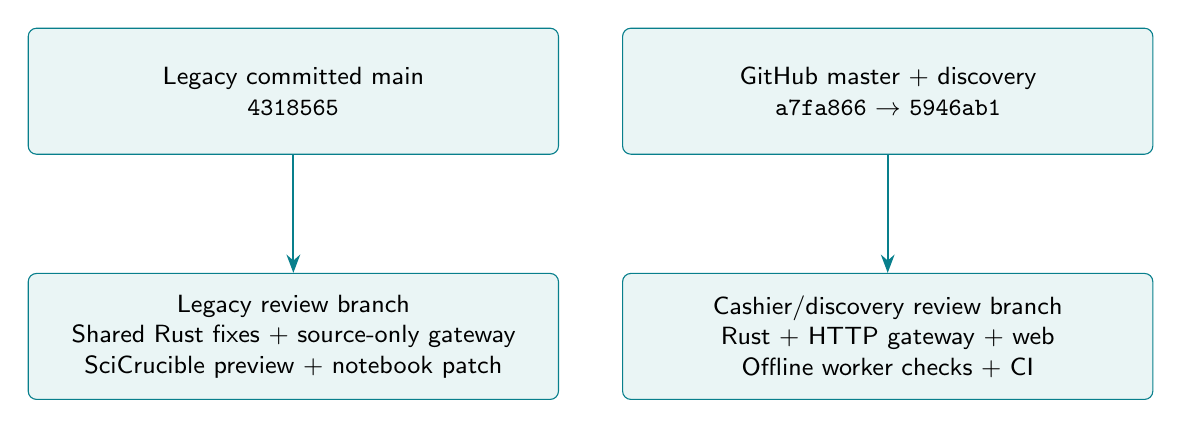
\begin{tikzpicture}[node distance=12mm,box/.style={draw=teal,rounded corners=3pt,fill=pale,align=center,text width=65mm,minimum height=16mm,font=\small\sffamily},arr/.style={-{Stealth},thick,draw=teal}]
\node[box] (a) {Legacy committed main\\\texttt{4318565}};
\node[box,right=8mm of a] (b) {GitHub master + discovery\\\texttt{a7fa866} $\rightarrow$ \texttt{5946ab1}};
\node[box,below=15mm of a] (c) {Legacy review branch\\Shared Rust fixes + source-only gateway\\SciCrucible preview + notebook patch};
\node[box,below=15mm of b] (d) {Cashier/discovery review branch\\Rust + HTTP gateway + web\\Offline worker checks + CI};
\draw[arr] (a)--(c);\draw[arr] (b)--(d);
\end{tikzpicture}
\end{center}
{\footnotesize\color{grey}Source: Git ancestry and component paths in the two review checkouts. This is an architecture/ancestry figure, not scientific performance data.}

\sub{What was included}
\begin{tabularx}{\textwidth}{@{}>{\raggedright\arraybackslash}p{30mm}Y@{}}\toprule
\textbf{Later line} & \texttt{improve/reliability-20261023}: starts at \texttt{5946ab1}; retains four reviewed discovery commits beyond remote master.\\\addlinespace
\textbf{Legacy line} & \texttt{improve/legacy-main-20261025}: starts at committed \texttt{4318565}; imports selected gateway source from the modified checkout and applies bounded fixes.\\\bottomrule
\end{tabularx}
Original checkouts were preserved. The legacy branch is \textbf{not a bulk snapshot} of the modified main tree. Notebook datasets, pilot records, scientific runs, environments and remaining uncommitted work were not imported.

\sub{Review coverage}
Primary Rust/HTTP/UI paths, offline worker tests, contract scaffolds, and modified-main notebook/fulfillment code. Alternate landing pages, all historical outputs, deployed services, provider accounts and scientific validity were not exhaustively audited. Changed source identities are recorded in each branch's \texttt{SOURCE\_MANIFEST.json}.
\newpage
\titleline{02 / IMPLEMENTED FIXES}{Protect the evidence boundary}
\begin{tabularx}{\textwidth}{@{}>{\raggedright\arraybackslash}p{31mm}Y@{}}\toprule
\textbf{Failure} & \textbf{Repair and evidence}\\\midrule
Forged signature & A weak identity public key and trivial signature passed verification. Strict Ed25519 verification now rejects the forgery; artifact/store/discovery regressions retain valid fixtures.\\\addlinespace
Store escape / overwrite & Canonical artifact IDs, filename/embedded-ID agreement, regular-file and symlink checks; complete bytes published atomically without replacement. Concurrent duplicate writes have one winner.\\\addlinespace
Worker identity / paths & DFT response IDs must match submitted IDs before cube writes. Digest filenames and exclusive creation prevent path escape and overwrite. Tests use fake workers.\\\addlinespace
Payment bypass & Arbitrary signature text no longer authorizes live x402 work. Requests fail closed and capability metadata says unavailable until real verification/settlement exists.\\\addlinespace
Wrong molecule & \texttt{C1CCCCC1} (cyclohexane) no longer matches \texttt{c1ccccc1} (benzene). Exact SMILES queries remain separate from normalized human labels.\\\addlinespace
Unbounded requests & Express IP trust rules replace raw forwarding headers. Rate state is bounded. MolADT process deadlines, output caps, concurrency caps and process-group cleanup have regression coverage.\\\addlinespace
Unhandled HTTP errors & Async rejection handling prevents revenue-log failures escaping Express 4. Containers run compiled JavaScript, without runtime \texttt{npx} downloads.\\\addlinespace
Checkout / fulfillment & Checkout API rejects unsupported minimum prices instead of silently increasing them. Legacy gateway adds serialized store operations and checkout-session idempotency.\\\bottomrule
\end{tabularx}

\sub{Make the interface describe its actual behavior}
Local state no longer claims submitted challenges, recomputation, wallet settlement or review completion. Fixture dates stay fixed. Checkout offers an intentional HTTPS link instead of an asynchronous popup that may be blocked. Legacy ORCID/submission/storage controls are explicitly unavailable previews.

\sub{Make build failures visible}
Both frontends enforce TypeScript validation. Two suppressed legacy errors were repaired: an absent icon export and a nonexistent post field. Unused network font downloads were removed. CI checks Rust, gateway tests/types/build, frontends, and the later branch's offline Python workers.

{\small\color{grey}Compatibility: store publication needs hard-link support and an operator-owned directory; \texttt{path\_for} is fallible. Repeated cube filenames fail instead of overwriting; use a fresh per-run output directory.}
\newpage
\titleline{03 / VERIFICATION}{Checks with explicit limits}
\begin{tabularx}{\textwidth}{@{}Y>{\raggedright\arraybackslash}p{43mm}>{\raggedright\arraybackslash}p{43mm}@{}}\toprule
\textbf{Check} & \textbf{Cashier / discovery} & \textbf{Legacy main}\\\midrule
Rust workspace, all features & 139 passed & 89 passed\\\addlinespace
Gateway regressions & 21 passed & 24 passed\\\addlinespace
Gateway types / compiled build & Passed & Passed\\\addlinespace
Frontend types / production build & Passed; 3 static pages & Passed; 43 routes\\\addlinespace
Checkout URL tests & 2 passed & Not applicable\\\addlinespace
Python 3.12 offline workers & 70 literature + 10 guard/stub tests passed & Not imported\\\addlinespace
Notebook authorization patch & Not applicable & 11 isolated checks passed\\\bottomrule
\end{tabularx}

\sub{How these results were obtained}
Rust used the installed macOS 15.2 SDK because the host's default SDK was incompatible with its linker. Initial dependency/cache/sandbox failures were resolved before the passing runs. Local Node was 25.9.0; CI targets Linux, Node 22 and Python 3.12. Local results do not establish hosted CI success.

Tests used fixtures and fake subprocesses. No scientific jobs, payment-provider transactions or deployments were performed. Independent inspection of the later branch found no blocking regression in the implemented fixes, with the reservations on the next page.

\sub{Notebook authorization patch: tested, not installed}
The separately modified notebook routes omit authorization on three mutation surfaces. The legacy delivery contains a patch, an isolated verifier and source/patch hashes. It adds session/role checks and actor binding. Original data and code were preserved; the patch has not been applied there.

\callout{The same isolated harness accepted a synthetic artifact with invalid signature, key and hashes after JSON comparison. It labelled it ready for manual release. No payout occurred. This defect remains unresolved.}

\sub{Publication and inspection limits}
Candidate changed files produced no matching live-key/private-key patterns in a scoped credential scan; this is not a whole-history secret audit. Runtime data and local secrets were excluded from the source import. Docker image execution, browser interaction, hosted uptime, DNS and provider integration were not verified. No browser surface was connected for interactive inspection.

The PDF is built from editable LaTeX. Final pages were rendered and inspected separately; visual PDF review does not imply browser verification.
\newpage
\titleline{04 / REMAINING WORK}{What the tests do not establish}
\begin{enumerate}\setlength{\itemsep}{9pt}
\item \textbf{Notebook trust and concurrency.} Add cryptographic verification and authorized signer checks before accepting a correction. Replace read-modify-rename state with transactions. Define access policy for public GET routes and complete authentication integration.
\item \textbf{Cached artifact authenticity.} Gateway cache files remain trusted operator inputs. The stricter Rust verifier does not automatically validate the HTTP cache read path; add verification at ingestion or serving.
\item \textbf{Worker bounds outside the gateway.} Direct Rust DFT execution still waits without time/output limits. Current gateway process limits protect MolADT invocation only.
\item \textbf{Payment qualification.} Live x402 settlement and live DFT remain unavailable. A configured Payment Link proves neither successful payment nor delivery. Legacy fulfillment storage is a single-process design. Old credit ledgers need explicit reconciliation; failures after redemption need manual entitlement recovery. Exactly-once delivery is not claimed.
\item \textbf{Contract scaffolds.} Reputation can be set publicly; governor authorization does not enforce quorum or voting. No contract deployment, governance readiness or financial authorization is implied.
\item \textbf{Operational evidence.} Run hosted CI and container smoke checks, then qualify one bounded payment-to-artifact path with provider test accounts. Reconcile source/data ownership before merging the two histories.
\end{enumerate}

\sub{Reproduce the software checks}
{\small\ttfamily
cargo test --workspace --all-features --locked\par
\vspace{3pt}
\# In services/api-gateway:\par
npm ci --ignore-scripts\par
npm run typecheck\par
npm test\par
npm run build\par
\vspace{3pt}
\# In web or SciCrucible\_v1:\par
npm ci --ignore-scripts\par
npm run typecheck\par
npm run build\par
}
\sub{Editable delivery}
\texttt{REVIEW.md}, \texttt{REVIEW.tex}, \texttt{BUILD.sh}, source manifests and verification receipts travel with the branches. The legacy notebook patch includes its own isolated verification script and a receipt explicitly preserving the unresolved-signature finding.
\end{document}
